\section{General properties of discrete Fourier transforms}
 Time series can be obtained from many sensors, for example; a pressure gauge in the water at at fixed depth, a range measurement from a laser or radar mounted on 
 a platform or ship, velocity from 
  underwater acoustic or electromagnetic systems, accelerometer in a floating system.  In the laboratory, it is common to measure 
  the surface elevation with resistive or capacitive wave gauges.  These times series thus consist of a signal $\zeta(t)$ or $p(t)$ sampled 
  at a fixed frequency  $f_s$, typically $1<f_s< 4$~Hz in the ocean,
and $f_s \sim  10~Hz$ or more in the laboratory because laboratory waves are generally  shorter and also, in the laboratory,  the internal memory and 
power consumption of instruments is less of an issue: either they are directly cabled to the acquisition system or the experiment is short enough.  
In general, it is very important that $f_s$ is at least 4 times the expected frequency of the signal of interest. Indeed, 
representing a cosine wave with only 4 points is already relatively coarse. As a result, some of the signal (the very short waves) is not resolved. 


Assuming we have such a series of discrete surface elevations
$\zeta(n)$ with $1\leq n\leq M$. The duration of the recording is 
$(M-1)/f_s$. All data processing softwares have a discrete Fourier transformation routine that will provide 
\begin{equation}
    Z_m= \frac{1}{M}\sum_{n=1}^{M} \zeta(n)  \mathrm{e}^{-2\mathrm{i}\pi
    (m-1)(n-1)/M}.\label{eq:Zm_def}
\end{equation}
\subsection{Spectral resolution}
For any frequency index $m$, the complex amplitude $Z_m$ is large when the signal $\zeta$ actually contains fluctuations at the frequency $f_m =(m-1)/M f_s$. The complex amplitudes contain both amplitude and phase information, i.e. $Z_m=|Z_m| \exp[\mathrm{i} \arg({Z_m})]$. The Fourier transform is simply a projection of the signal onto the elementary functions that are the complex exponentials, or if you prefer sines and cosines, with all frequencies $f_m =(m-1)/M f_s$ where $m$ goes from 1 to M. We note that the difference between frequencies $f_m$ and $f_{m+1}$ is the spectral resolution $df = f_s / M$. Because $f_s$ is the inverse of the sampling interval $dt$, we have $df = 1/(M dt)$, which is the inverse of the record duration. Namely, the frequency resolution is the same as the lowest frequency which is at $m=2$, and it such that the lowest period equals the record duration.  We recall that $m=1$ gives the average value of the signal. 




\subsection{Nyquist frequency}
The decomposition of a discretized real signal with $M$ pieces of information into $M$ frequencies cannot produce $M$ amplitudes and frequencies that are independent, that would be $2M$ pieces of information. Indeed, the frequencies from $M/2 f_s$ to $M f_s$ do contain the same information as those between $0$ $(M/2-1) f_s$, as shown in figure \ref{fig:anaspec:spectreDFT}.
%%%%%%%%%%%%%%%%%%%%%%%%%%%%%%%%%%%%%%%%%%%%%%%%%%%%%%%%%%%%%%%%%%%%%%%%%%%%
\begin{figure}
\centerline{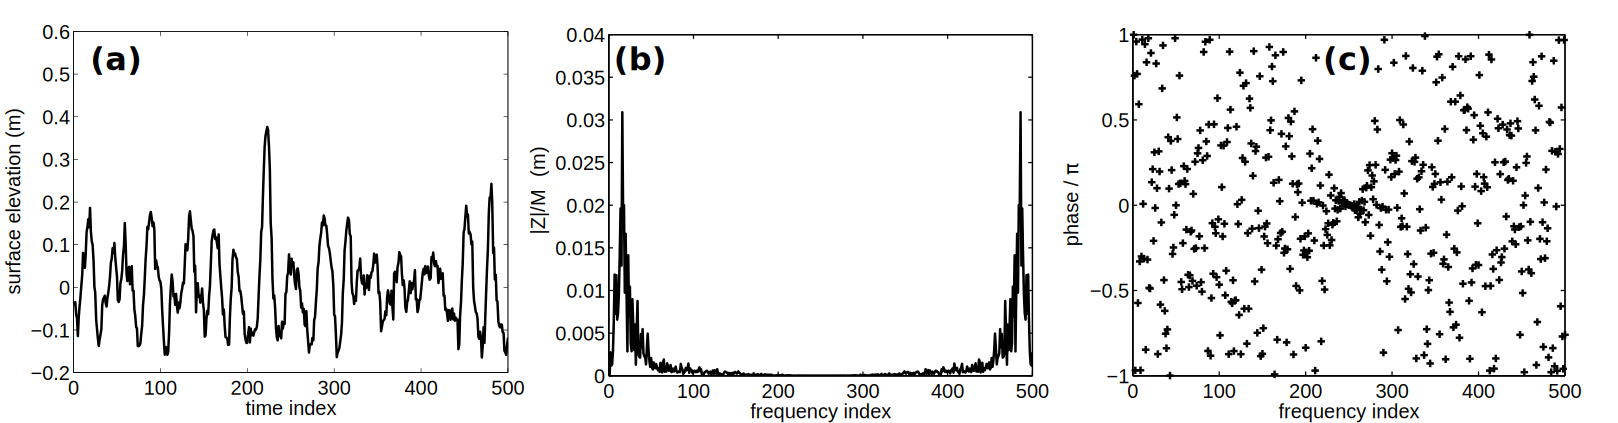
\includegraphics[width=0.9\textwidth]{FIGURES/spectra_DFT.pdf}}
%\vspace{3.64in}
\caption{(a) Example of surface elevation time series sampled at 12~Hz, (b) Discrete Fourier transform amplitude of the signal, and (c) phase of the same signal.} \label{fig:anaspec:spectreDFT}
\end{figure}
%%%%%%%%%%%%%%%%%%%%%%%%%%%%%%%%%%%%%%%%%%%%%%%%%%%%%%%%%%%%%%%%%%%%%%%%%%%%

With the definition given by eq. (\ref{eq:Zm_def}),  $Z_m=
\overline{Z_{M+2-m}}$, where the overbar is the complex conjugate, so that the modululs of the spectrum is symmetric around  $m=M/2$. This index $M/2$ corresponds to the Nyquist frequency 
$f_N=f_s/2 = M/2 df$. The symmetry means that above $f_N$ there is no new information. In other words, $f_N$ is the highest resolvable frequency. At this Nyquist frequency, a cosine wave is only represented by 2 points over a period. 

%We note that for stationary random variables that are quadratically integrable, i.e. all practical physical signals, the ratio $dZ(m) \overline{dZ(m)} / df$ goes to %$F(f)$ when $M$ goes 
%to infinity, i.e.  $f_s$ goes to zero, provided that  we keep constant 
%$f=(m-1)f_s/N$.  The increment
%$df=f_s/(N-1)$ is the spectral resolution, namely the frequency difference that can be resolved. The inverse of this resolution 
%$1/df$ is equal to the length of the recorded signal.

The continuous spectral density   $F(f)$ is obtained in the limit when the spectral resolution $df$ goes to zero of the following expression
\begin{equation}
    F(f=(m-1)f_s/M)  = 2  \frac{Z_m \overline{Z_m}}{df}.
\end{equation}
The factor 2 comes from the combination of positive and negative frequencies in the interval  $[0,  f_N]$. That definition is 
called the  single-sided spectrum. For some applications it may be convenient to keep the double-sided spectrum defined without this factor 2, 
for $f$ in the range $[0 , 2 f_N]$ or $[-f_N ,  f_N]$. 
In practice, the zero spectral resolution is never achieved because it corresponds to an infinitely long record. We are therefore stuck to finite 
spectral resolutions $df$, and thus a discrete spectrum sampled at $df$, corresponding to record lengths over which the random variable of interest is stationary. 


\subsection{Co-spectra}
In the same manner, we can  define the co-spectrum of two variables $a$ and $b$ having Fourier transforms $dA$ and $dB$, 
\begin{equation}
    C_{ab}(f=(m-1)f_s/M)  = \frac{A_m \overline{B_m}}{df} = P(f) +\mathrm{i}Q(f),
\end{equation}
where $P$ and $Q$ are real numbers, the co-spectra in phase and quadrature. 

We note that the product of two Fourier transforms is the Fourier transform of the convolution of the two functions. When these two functions are the same,
this result tells us that the spectrum is the Fourier transform of the auto-correlation function. When the two functions are different, the co-spectrum
is the Fourier transform of the correlation function. 

\section{Spectra from time series}
\subsection{Filtering of data and aliasing}
For any physical
parameter, the complex amplitude at a frequency above $f_N$ is the complex conjugate of the amplitude at a frequency below $f_N$: $dZ(N-m)=\overline{dZ(m)}$. 
In other words, the energy above the Nyquist frequency is aliased at  lower frequencies. This is one reason for applying a low-pass filter before the Fourier transform, in order to remove signals that would otherwise be aliased. 


%Il faut toujours bien r�fl�chir � la mani�re dont les donn�es sont filtr�es avant leur 
%�chantillonnage. Quand on mesure des vitesses toutes les dix minutes, est-ce une mesure instantan�e 
%une moyenne sur une, deux ou dix minutes? En effet les vitesses mesur�es contiendront alors 
%le courant moyen (par exemple caus� par la mar�e) mais aussi, si aucune moyenne n'est faite, les 
%fluctuations associ�es aux vagues et qu'il peut �tre tr�s d�licat de supprimer a post�riori. 

For example, a signal of period 1~s sampled every second ($f_s = 1$~Hz) is constant.  In general, any signal with frequency higher 
than the Nyquist frequency gives an apparent frequency in the range 
$[0 f_s/2]$, with a value obtained by folding back the spectrum along a vertical line at  $f=f_s/2$ or $f=0$ as many times as necessary, until 
 falling in $[0 f_s/2]$. Figure \ref{aliasing} shows an example of a true signal (in red) with frequency at  9/10 which gives  1-9/10=1/10 by aliasing. 
This is well known problem in oceanography in the case of the measurement of tides from satellite data. 
In the case of ocean waves, it is really necessary to measure waves with a sampling frequency that is at least 4 times the dominant frequency.  
%%%%%%%%%%%%%%%%%%%%%%%%%%%%%%%%%%%%%%%%%%%%%%%%%%%%%%%%%%%%%%%%%%%%%%%%%%%%
\begin{figure}[htb]
\centerline{\includegraphics[width=0.5\textwidth]{FIGURES/AliasingSines.pdf}}
%\vspace{3.64in}
\caption{Example of spectral aliasing. A signal with period 10/9, in red, and sampled with a step of 1 (black dots) 
gives an apparent period of  10, in blue. (Moxfyre, wikimedia commons).} \label{aliasing}
\end{figure}
%%%%%%%%%%%%%%%%%%%%%%%%%%%%%%%%%%%%%%%%%%%%%%%%%%%%%%%%%%%%%%%%%%%%%%%%%%%%

In practice the high frequency roll-off of the wave spectrum, for $f > f_p$ in particular for pressure or velocity at the ocean floor, means that this 
filtering may not be necessary for the surface elevation. 
Figure \ref{fig:anaspec:timeseries} shows an example of the filtering of a surface elevation record and its impact on the spectrum. Here the filter helps in reducing 
the noise associated with the measurement method. 
%%%%%%%%%%%%%%%%%%%%%%%%%%%%%%%%%%%%%%%%%%%%%%%%%%%%%%%%%%%%%%%%%%%%%%%%%%%%
\begin{figure}[htb]
\centerline{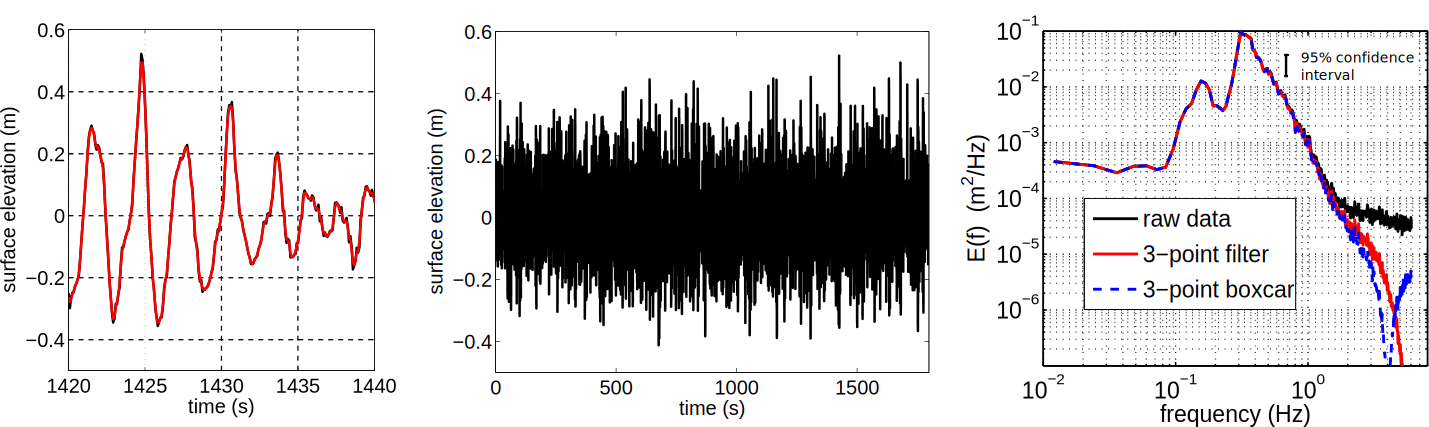
\includegraphics[width=\textwidth]{FIGURES/timeseries.pdf}}
%\vspace{3.64in}
\caption{Example of surface elevation measured by stereo-video from the Katsiveli platform, in 20~m depth, on Octoebr 4, 2011 \citep[see][for further detailed analysis of this dataset]{Leckler&al.2015,Aubourg&al.2017}.  (a) small piece of record around $t= 1430~s$ with (red) and without (black) a 3-point smoothing filter  (b) full record (1780~s) (c) spectra of the time series with different filters applied.} \label{fig:anaspec:timeseries}
\end{figure}
%%%%%%%%%%%%%%%%%%%%%%%%%%%%%%%%%%%%%%%%%%%%%%%%%%%%%%%%%%%%%%%%%%%%%%%%%%%%
The worst filter is clearly the boxcar (or moving average) filter with equal weight given to the consecutive data values, this does not suppress very well the shortest components.  


\subsection{Windows, Gibbs phenomenon and averaging}
The discrete Fourier transform of signal $\zeta$ that takes values at locations 1 to N, corresponds to the Fourier transform of a periodic signal that would 
repeat itself with $\zeta(n+m M) = \zeta (n)$ for any $n$ and $m$. If 
$\zeta(1)\neq \zeta(M)$, then this periodic function has a sharp jump from $\zeta(M)$ to $\zeta(M+1)$. Such a jump 
can give a strong spectral signature, all across the spectrum. 


This artifact is known as the Gibbs phenomenon, and it 
is generally removed by multiplying the signal  $\zeta(n)$ by a window function $W(n)$ which goes to zero or very small values for both 
$n=1$ and $n=N$. Obviously the spectrum of $\zeta(n) \times W(n)$ is different from the spectrum of $\zeta(n)$. The first obvious effect is that 
the variance of the signal has been reduced by a factor that is the average of $W^2$. That is easily corrected for.




Let use the time series shown in figure \ref{fig:anaspec:timeseries}.b. We first start with a small piece of only 1000 points. The original time series, in black 
in figure \ref{fig:anaspec:spectre1}.a gives the power spectral density in figure {fig:anaspec:spectre1}.b. If the time series is brought to zero at both ends (in red) by multiplying with a Hann window, then the spectrum is transformed. However, because of the random fluctuations of the spectral estimates this is not obvious.
Indeed waves are random and the surface elevation is nearly-Gaussian. As a result, the complex Fourier amplitudes are also random and Gaussian, so that they modulus, which is the power spectral density has the shape of a  $\chi^2_n$ distribution with $n=2$ degrees of freedom. Because the $\chi^2_n$ distribution has a mean of $n$, the distribution of estimates $\widehat{E}(f)$ of the spectrum, once normalized by the mean spectrum $E(f)$ follows the rescaled $\chi^2_n$ disitribution, with a mean equal to 1. 

%%%%%%%%%%%%%%%%%%%%%%%%%%%%%%%%%%%%%%%%%%%%%%%%%%%%%%%%%%%%%%%%%%%%%%%%%%%%
\begin{figure}[htb]
\centerline{\includegraphics[width=\textwidth]{FIGURES/spectra1.pdf}}
%\vspace{3.64in}
\caption{(a) First 1000 points of time series shown in  (\ref{fig:anaspec:timeseries}).b, with (red) and without (black) multiplication by a Hann window. 
(b) Resulting spectra (c) Average spectra using Welch's method with 21 independent windows and thus 42 degrees of freedom.} \label{fig:anaspec:spectre1}
\end{figure}
%%%%%%%%%%%%%%%%%%%%%%%%%%%%%%%%%%%%%%%%%%%%%%%%%%%%%%%%%%%%%%%%%%%%%%%%%%%%
 Using figure \ref{table_chi2}, we find that the expected ratio of the lower and upper bound of a 95$\%$ confidence interval is 146. This number is the ratio of  $\chi^2_{2,0.975}$�and  $\chi^2_{2,0.025}$, that give the probabilities that $\chi^2_{n} > \chi^2_{n,\alpha}$ is equal to the acceptance threshold $\alpha$. 
%%%%%%%%%%%%%%%%%%%%%%%%%%%%%%%%%%%%%%%%%%%%%%%%%%%%%%%%%%%%%%%%%%%%%%%%%%%%
\begin{figure}
\centerline{\includegraphics[width=\textwidth]{FIGURES/table_chi2.png}}
%\vspace{3.64in}
\caption{Table of $\chi^2$ distributions. This table gives the confidence intervals
for the estimation of spectra with 
$n=2 N$ degrees of freedom, where $N$ is the number of independent spectra used.} \label{table_chi2}
\end{figure}
%%%%%%%%%%%%%%%%%%%%%%%%%%%%%%%%%%%%%%%%%%%%%%%%%%%%%%%%%%%%%%%%%%%%%%%%%%%%


For an expected value  $\widehat{E}$, the  Gaussian statistics theory predicts a 95\% probability that the estimate of $E(f)$ is in the range $[E_1, E_2]$ with $E_1=\widehat{E} \times 0.0506/2 $ and  $E_2=\widehat{E} \times 7.38/2$, where 0.0506 and 7.38 are the values for which the $\chi^2$ cumulative probability function for 2 degrees of freedom is $\alpha=0.975$ and $\alpha=0.025$, respectively as given \ref{table_chi2}. In other words, the random fluctuations of the spectrum estimated by a single Fourier transform spans more than two orders of magnitude. 

That is fairly annoying. There are two ways to reduce this uncertainty: the first, which is most easily done in the laboratory is to run more experiments, repeating the same conditions, with random wave phases, and average the results. For measurements in the field, this is the same as processing a longer time series, but it only makes sense if the conditions are stationary: same wind, same wave age, same current, etc. In practice, this stationarity constraints limits the length of records from half an hour to a few hours. As we average $N$ spectra together, the number of degrees of freedom increases to $2N$. Here we have used 21 independent spectra, and we get an uncertainty that narrows like $1/\sqrt{N}$ for large $N$. For 20 spectra, the ratio $E_2/E_1$ is $59.34/34.43\simeq 1.7$. As $N$ increases, the spectral resolution becomes coarser.

Because the Hann window practically removes part of the data, \cite{Welch1967} has defined a method in which the windows are shifted by half their length, as shown in figure \ref{fig:anaspec:spectre31}.a. The lower panel shows the 21+20 spectra estimated, and the average result.  
%%%%%%%%%%%%%%%%%%%%%%%%%%%%%%%%%%%%%%%%%%%%%%%%%%%%%%%%%%%%%%%%%%%%%%%%%%%%
\begin{figure}
\centerline{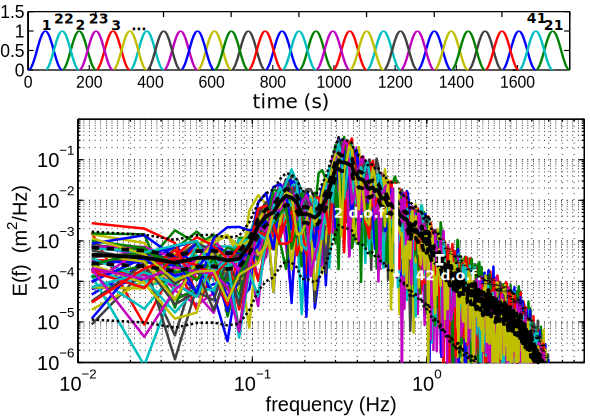
\includegraphics[width=0.9\textwidth]{FIGURES/spectra_31.pdf}}
%\vspace{3.64in}
\caption{(a) Succession of the Hann windows applied to the data, with 21 independent windows and 20 overlapping windows, from number 22 to 41. The solid line is the mean spectrum and the dotted and dashed line show the expected 95\% confidence intervals for 2 and 42 degrees of freedom. 
� 95\%.} \label{fig:anaspec:spectre31}
\end{figure}
%%%%%%%%%%%%%%%%%%%%%%%%%%%%%%%%%%%%%%%%%%%%%%%%%%%%%%%%%%%%%%%%%%%%%%%%%%%%

Another method that is almost equivalent to Welch's is the smoothing of the spectrum, also known as band-averaging. Because the Fourier transform of a shorter 
window has a coarser resolution, both methods effectively trade off the spectrum accuracy against the spectral resolution. An extension of such methods is the use of wavelet transforms \citep[e.g.][]{Liu&Babanin2004} which aims at localizing events in both time and frequency. 

Whatever the choice of method, without any prior knowledge on the signal, the product of the spectra uncertainty and the square root of the frequency uncertainty remains constant. Thus the optimal choice of $df$ is up to the user. For wind seas, the typical relative width of the spectrum is 0.1, and for a typical peak period of 0.1~Hz, resolving the peak requires $df < 0.01$~Hz. For swells one may like to have an even narrower frequency resolution.  In the example above, $df=0.012$~Hz is 
enough for the relatively short wind sea found in the Black Sea. 

\subsection{Interpretations and further developments}
The general idea of spectral analysis is to decompose a signal into its basic constituents. If waves were indeed linear, the Fourier components would be truly independent and the spectrum would give the energy of different wave components. In practice, there is a significant level of nonlinearity, which actually dominates the frequency spectrum $E(f)$ at frequencies above 3 to 4 times the wind sea peak \citep[e.g.][]{Leckler&al.2015}. As a result, the interpretation of these high frequencies ($f > 1$~Hz in the example above) as the energy of linear waves is wrong. Several methods have been developed to try to separate linear and non-linear components, including higher order analysis \citep{Hasselmann&al.1963} which is illustrated in chapter \ref{ch_surf}. This question has inspired other nonlinear methods, such as the Empirical Mode Decomposition method by \cite{Huang&al.1998}.


\section{Spectral analysis of directional buoy data}
\subsection{Case of 3-axis displacements or accelerations}
We have seen in section  \ref{sub:transfer} that the spectrum of $x$-component velocity  at the ocean bottom 
is given from the surface elevation spectrum multiplied by a transfer function,
\begin{equation}
    E_{Ux} \left( f,\theta \right)  = \frac{\sigma^2 \cos^2 \theta}{\sinh^2 (kD)} E\left( f,\theta
    \right)\label{EUX }.
\end{equation}
%et le module moyen de la vitesse (en moyenne quadratique) pr�s du fond vaut,
%\begin{equation}
%    U_{\mathrm{b,rms}} = \left[\int_0^{\infty} \int_0^{2 \upi} \frac{\sigma^2}{\sinh^2
%    (kD)} E\left( f,\theta \right){\mathrm d}\theta
%    {\mathrm d}f \right]^{1/2}
%\end{equation}

The same method applies to spectra of displacements, velocity and slopes at the sea surface. 
For a water particle at the surface, the spectra of displacement in the three directions are given by  (\ref{xi3}),
\begin{eqnarray}
    E_{x} ( f)  & = &  \frac{1}{\tanh^2(kD)} \int_0^{2 \upi} E\left( f,\theta \right)\cos^2 \theta {\mathrm
    d}\theta \\
    E_{y} ( f)  & = &  \frac{1}{\tanh^2(kD)} \int_0^{2 \upi} E\left( f,\theta \right)\sin^2 \theta {\mathrm
    d}\theta \\
   E_{z} ( f)  & = &  \int_0^{2 \upi} E\left( f,\theta \right) {\mathrm
    d}\theta.
\end{eqnarray}
We note that this last spectrum is the usual elevation spectrum $E(f)$, also called heave spectrum, with a minor modification due to the fact that it is not 
obtained at a fixed position $(x,y)$ but at a positions that moves with $x$ and $y$. As a result, the shape of the waves and the shape of the spectrum are modified, with a strong reduction in the contribution of nonlinear harmonics: a surface buoy signal looks much more linear than a wave staff or stereo video record. 

The co-spectra of horizontal and vertical displacements are 
\begin{eqnarray}
    C_{xz} ( f)  & = &  \frac{\mathrm i}{\tanh(kD)} \int_0^{2 \upi} E\left( f,\theta \right)\cos \theta {\mathrm
    d}\theta, \label{Exz}\\
    C_{yz} ( f)  & = &  \frac{\mathrm i}{\tanh(kD)} \int_0^{2 \upi} E\left( f,\theta \right)\sin \theta {\mathrm
    d}\theta .\label{Eyz} \\
    C_{xy} ( f)  & = &  \frac{1}{\tanh^2(kD)} \int_0^{2 \upi} E\left( f,\theta \right)\sin \theta \cos \theta {\mathrm
    d}\theta .\label{Exy}
\end{eqnarray}
These co-spectra are thus related to the mean direction and directional spread, through the directional moments introduced in section  \ref{sub:param}
\begin{eqnarray}
    a_1 ( f)  & = &  \int_0^{2 \upi} E\left( f,\theta \right)\cos \theta {\mathrm
    d}\theta, \\
    b_1 ( f)  & = &   \int_0^{2 \upi} E\left( f,\theta \right)\sin \theta {\mathrm
    d}\theta,  \\
    a_2 ( f)  & = &  \int_0^{2 \upi} E\left( f,\theta \right)\cos (2\theta) {\mathrm
    d}\theta, \\
    b_2 ( f)  & = &   \int_0^{2 \upi} E\left( f,\theta \right)\sin (2 \theta) {\mathrm
    d}\theta.
\end{eqnarray}


To summarize, starting from the displacement time series  $x(t)$, $y(t))$ and $z(t)$ one obtains the 
spectra and co-spectra  $C_{xx}(f)$,  $C_{yy}(f)$,  $C_{zz}(f)$,  $C_{xz}(f)$, $C_{yz}(f)$ , $C_{xy}(f)$.
Using $\cos(2 \theta)=\cos^2(\theta) - \sin^2(\theta)$ and $\sin(2 \theta)=2 \sin \theta \cos\theta$, they give the following directional moments, in which $\Im $ stands for the imaginary part, 
\begin{eqnarray}
  a_1 ( f) &=&-\Im (C_{xz}(f))/\left[C_{zz}(f) \left(C_{xx}(f)+C_{yy}(f)\right)\right] \\
  b_1 ( f) &=&-\Im (C_{xy}(f))/\left[C_{zz}(f) \left(C_{xx}(f)+C_{yy}(f)\right)\right] \\
  a_2 ( f) &=&(C_{xx}(f)-C_{yy}(f))/(C_{xx}(f)+C_{yy}(f)) \\
  b_2 ( f) &=&2 C_{xy}(f) /(C_{xx}(f)+C_{yy}(f))  \\
\end{eqnarray}
from which we get directional parameters, with $\mod$ the modulo operator, 
\begin{eqnarray}
  \theta_{1}(f) &=&  \mod( 270.- \mathrm{atan2}(b1,a1)\times 180/\pi, 360)\\
  \sigma_{1}(f)&=&\left[2\left(1 - \sqrt{a_1^2(f) + b_1^2(f)} \right)\right]^{0.5}\times 180/\pi \\
  \theta_{2}(f) &=&  \mod( 270.- 0.5 \mathrm{atan2}(b2,a2)\times 180/\pi, 360)\\
  \sigma_{2}(f)&=&\left[0.5\left(1 - \sqrt{a_2^2(f) + b_2^2(f)} \right)\right]^{0.5}\times 180/\pi
\end{eqnarray}


These 4 parameters can be used in statistical estimators to obtain the directional spectrum $E(f,\theta)$. A commonly used estimator 
is the Maximum Entropy Method of \cite{Lygre&Krogstad1986}. See also the review by \cite{Benoit&al.1997}.

\subsection{Case of other systems with 3 variables or more}
in the above method, we can replace $x$ and $y$ by the slopes $\partial \zeta / \partial x$  and $\partial \zeta / \partial y$ as done in the pitch-and-roll buoys 
developed by \cite{Cartwright&Smith1964} and still widely used. For example, most of the 3-m discuss buoys operated by the U.S. National Data Buoy Center are based 
on this measurement \citep{Steele&al.1992}. Also, the horizontal 
velocities at any given level, $(u,v)$. These give access to the heave spectrum $E(f)$ and the same directional moments $a_1$, $b_1$, $a_2$ and $b_2$. 

In order to go beyond these first 5 parameters, one can built an array of instruments. The cloverleaf buoy of \cite{Mitsuyasu&al.1975} was such an attempt, and arrays of pressure gages or lasers have been routinely used. Today's optical techniques \citep{Benetazzo2006,Fedele&al.2013,Laxague&al.2015} are other ways to get to more details about the sea surface.


\section{Some links between spectral and wave-by-wave analysis}
The spectrum $E(f)$ gives the distribution of the surface elevation variance as a function of time scales. As discussed in chapter \ref{ch1}, one can also chop the 
signal in individual waves and study the statistics of their properties. 
A model for the sea surface elevation could be a signal of constant amplitude with a random frequency modulation. In that case, \cite{Woodward1952}'s theorem 
tells us that the spectrum of the signal is the distribution of its frequencies $P_f(f-f_c)$ where $f_c$ is the carrier frequency,
\begin{equation}
    E(f) = \frac{a^2}{2}P_f(f-f_c).
\end{equation}

Extension of that theorem by \cite{Blachman&McAlpine1969} with an additional amplitude modulation makes it applicable to ocean waves.  As  shown by  \cite{Elfouhaily&al.2003} the spectrum is then given by the joint probability distribution of wave heights and periods $P(a,f)$ with $a=H/2$ and $f=1/T$. 
Separating linear (naked) and full (dressed) spectra, \cite{Elfouhaily&al.2003} showed that the peak region is dominated by linear components 
\begin{equation}
    E_{\mathrm bare}(f) = \frac{1}{2}\int a^2 P(a,f) da.
\end{equation}

At high frequency the nonlinear contributions dominate the spectrum which can be interpreted as fast modulations of the short components. Taking into account that 
effect leads to asymetries $\alpha$ et $\beta$
(see figure \ref{Asymetrie_Elf}), and the dressed spectrum
\begin{equation}
    E_{\mathrm{dressed}}(f) =  E_{\mathrm nu}(f) +\frac{1}{2}\left[ \int \alpha^2 P(\alpha,f/2)
    da+ \int \beta^2 P(\beta,f/2) da\right] \simeq E(f)
\end{equation}
%%%%%%%%%%%%%%%%%%%%%%%%%%%%%%%%%%%%%%%%%%%%%%%%%%%%%%%%%%%%%%%%%%%%%%%%%%%%%%%%%%%%%
\begin{figure}
\centerline{\includegraphics[width=0.6\textwidth]{FIGURES/Asymetrie_Elf.pdf}}
%\vspace{3.64in}
  \caption{Definition of parameters $M$ ,$m$, $T_1$ et $T_2$ used to estimate the amplitude  $a=(M-m)/2$, period $T=T_1+T_2$, vertical asymetry  $\alpha=(M+m)/2$  and horizontal asymetry $a\pi(T_1-T_2)/(T_1+T_2)/2$ (from \cite{Elfouhaily&al.2003}, \copyright Elsevier).
   Here $m<0$, because $m$ is defined as the trough level between two up-crossing zeros that define the start and end of the wave.} \label{Asymetrie_Elf}
\end{figure}
%%%%%%%%%%%%%%%%%%%%%%%%%%%%%%%%%%%%%%%%%%%%%%%%%%%%%%%%%%%%%%%%%%%%%%%%%%%%%%%%%%%%%%%%%%%


